\section{ZMPと支持多角形による安定性評価}

二足歩行ロボットの安定性を評価する代表的な指標として，ZMP（Zero Moment Point）が広く用いられている．ZMPとは，床反力によるモーメントがゼロとなる床面上の点であり，この点が支持多角形の内部に存在する場合，ロボットは転倒しないと考えられる．

支持多角形は，ロボットが床と接触している支持脚の接地点を結んで形成される領域である（\cref{fig:foot_shape}）．両脚支持期（Double Support: DS）では支持多角形は広く，片脚支持期（Single Support: SS）では支持多角形は支持脚足裏の領域に限定される．このため，SSでは安定性の余裕が小さく，制御がより困難となる．

ZMPは，CoMの運動と密接に関係しており，CoMの加速度や高さの変化によってその位置が変動する．したがって，ZMPを支持多角形内に保つことは，CoM運動を適切に制御することと等価であると捉えることができる．

\begin{figure}[htbp]
  \centering
  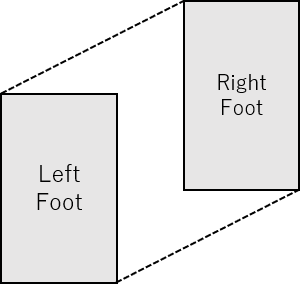
\includegraphics[width=0.3\linewidth]{images/foot.png}
  \caption{支持多角形}
  \label{fig:foot_shape}
\end{figure}